\documentclass[border=10pt,crop,tikz,convert={outext=.svg,command=\unexpanded{pdf2svg \infile\space\outfile}},multi=false]{standalone}
\usepackage{lmodern}
\usepackage{graphics}
\usepackage{tikz}
\usetikzlibrary{positioning}  % use: above left of, etc
\usetikzlibrary{arrows}
\usetikzlibrary{babel}
\usetikzlibrary{automata}
\usetikzlibrary{shapes, snakes}
\usetikzlibrary{positioning, fit, calc}
\usetikzlibrary{decorations.pathreplacing,calligraphy}

\usepackage{varwidth}
\usetikzlibrary{shapes.multipart}


\usepackage{pgfplots}
\pgfplotsset{compat=newest}
\usepackage{pgf}
\newcommand{\drawge}{-- (rel axis cs:1,0) -- (rel axis cs:1,1) -- (rel axis cs:0,1) \closedcycle}
\newcommand{\drawle}{-- (rel axis cs:1,0) -- (rel axis cs:0,0) -- (rel axis cs:0,1)  \closedcycle}
\pgfplotsset{samples=1000}
\pgfplotsset{axis on top}
\usepgfplotslibrary{fillbetween}


\pgfrealjobname{logo}
\begin{document}

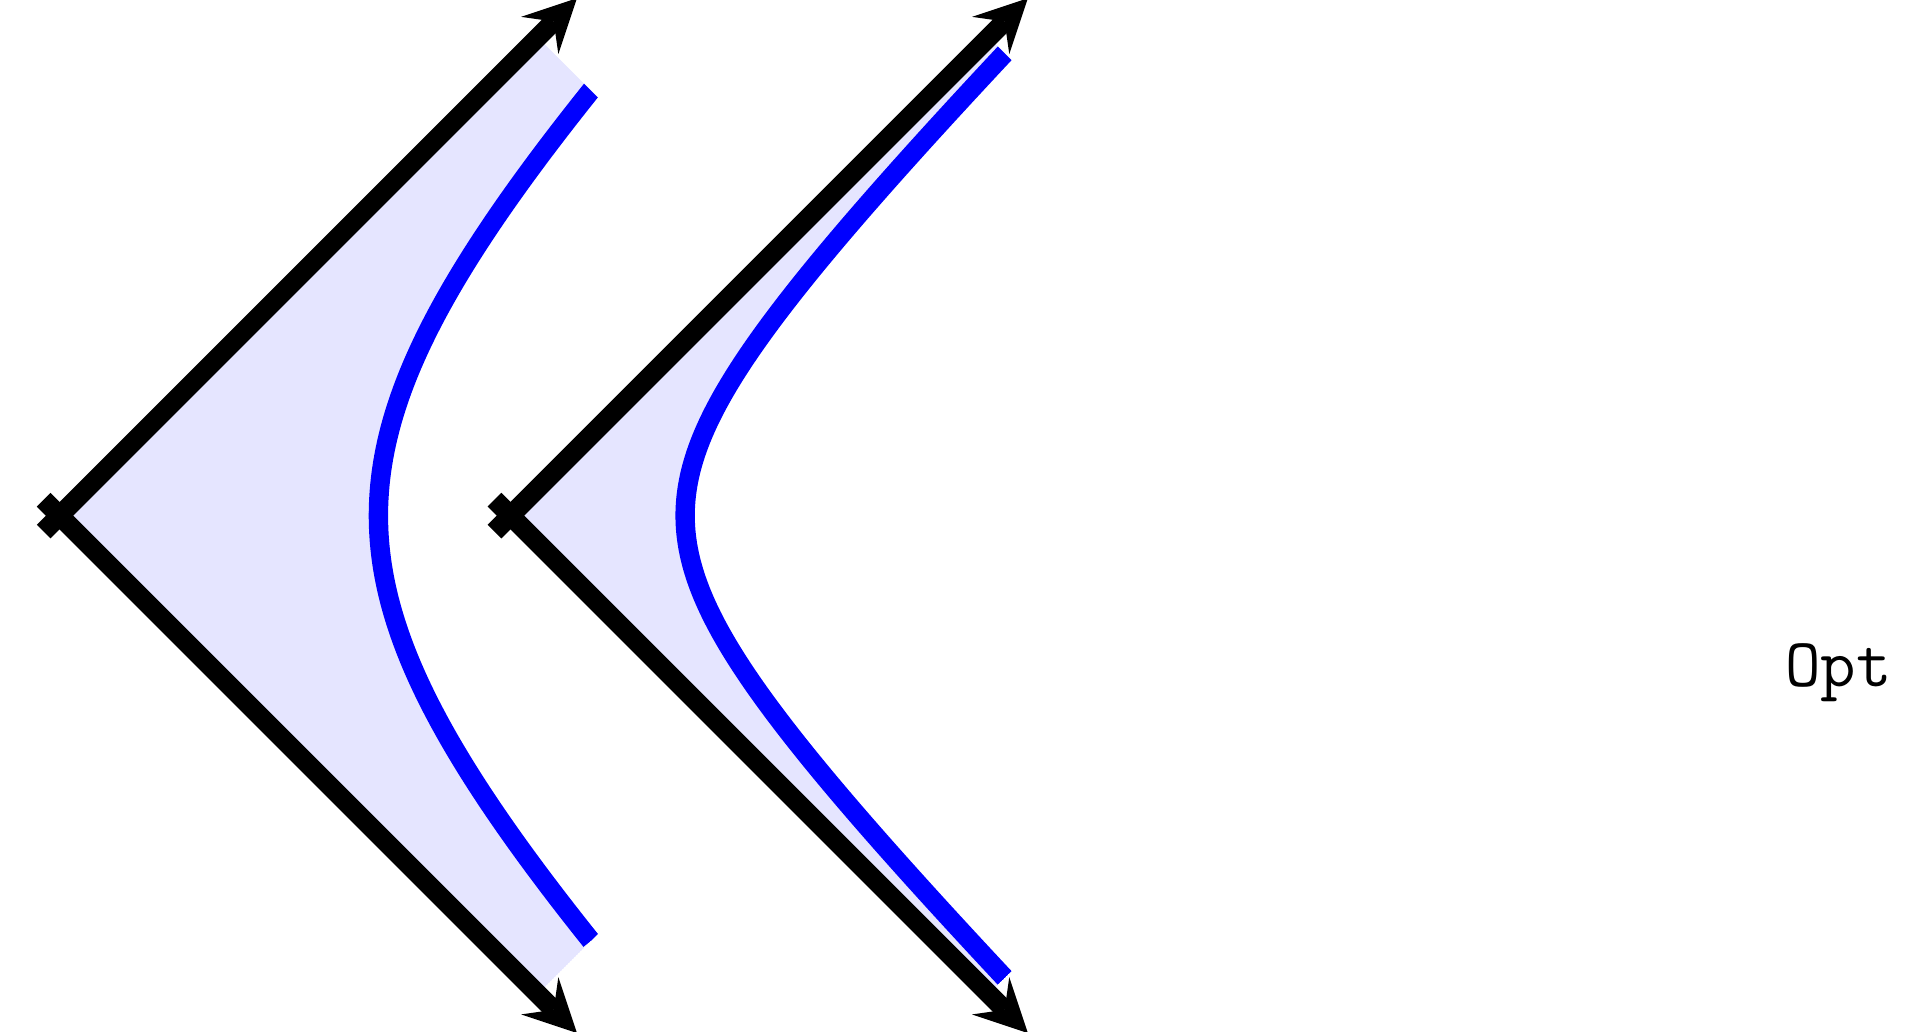
\begin{tikzpicture}%[every node/.style={inner sep=1cm,outer sep=1cm}]
  \begin{axis}[
    outer sep=-5pt,
    width=\textwidth, axis equal image,
    xmin=-0.1,xmax=3.0,
    ymin=-0.1,ymax=3.0,
    ticks=none,
    axis x line=center, axis y line=center,
    xlabel style={below right},
    ylabel style={above left},
    axis line style = {line width = 7pt, shorten >=-20pt},
    rotate=-45
    ]
    \addplot[name path=psi, id=scholtes1,smooth,domain=0:3, range=0:3, line width = 7pt, color=blue,restrict y to domain=0:100] {1.0/x};
    \addplot[name path=paxis, domain=0:3] {0};
    %\path[name path=paxis] (0.5,0) -- (1.5,0);
    \addplot[blue!10] fill between[of=paxis and psi, reverse=true];
    %\addplot[blue!10] fill between[of=paxis2 and psi];
  \end{axis}

  \begin{axis}[
    outer sep=5pt,
    width=\textwidth, axis equal image,
    xmin=-0.1,xmax=3.0,
    ymin=-0.1,ymax=3.0,
    ticks=none,
    axis x line=center, axis y line=center,
    xlabel style={below right},
    ylabel style={above left},
    axis line style = {line width = 7pt, shorten >=-20pt},
    rotate=-45,
    at={(200,0)}
    ]
    \addplot[name path=psi, id=scholtes1,smooth,domain=0:3, range=0:3, line width = 7pt, color=blue,restrict y to domain=0:100] {0.3/x};
    \addplot[name path=paxis, domain=0:3] {0};
    %\path[name path=paxis] (0.5,0) -- (1.5,0);
    \addplot[blue!10] fill between[of=paxis and psi, reverse=true];
    %\addplot[blue!10] fill between[of=paxis2 and psi];
  \end{axis}
  \node[] at (23,-2) {\texttt{\fontsize{400pt}{300pt}\selectfont Opt}};
\end{tikzpicture}

\end{document}`
%%% Local Variables:
%%% mode: LaTeX
%%% TeX-command-extra-options: "-shell-escape"
%%% TeX-master: t
%%% End:
